\section{Algorithm Design and Implementation}

\subsection{Zero Run Analysis Explanation}
The \texttt{AnalyzeZeroRun} procedure employs three fundamental constraints to verify potential
zero runs in the binary expansion of $\sqrt{2}$:
\begin{enumerate}
    \item \textbf{Integer Constraint (\texttt{integerOK})}: This constraint examines whether the numerical
    representation is valid in binary form. It verifies that our approximation produces
    well-defined binary digits without ambiguity.
    \item \textbf{Next Bit Constraint (\texttt{nextBitOK})}: This ensures the mathematical validity of the
    sequence’s termination. The constraint confirms that each zero run must eventually
    terminate with a 1, which is a fundamental property of $\sqrt{2}$’s binary expansion.
    \item \textbf{Square Root Constraint (\texttt{sqrt2OK})}: This provides mathematical verification that
    our approximation accurately represents $\sqrt{2}$. The constraint ensures that when we
    square our approximated value, it closely matches 2 within our defined error bounds.
\end{enumerate}

These constraints work in concert to establish rigorous criteria for valid zero runs. As
demonstrated in the paper’s analysis, when $k$ (the length of a zero run) exceeds $\log_2(n)$ at
position $n$, these constraints become fundamentally incompatible, providing strong evidence
for the paper’s central conjecture.

\subsection{Algorithm Workflow}
To improve accessibility, we present a high-level pseudocode summary of the algorithm:

\begin{algorithm}[H]
\caption{Zero Run Analysis Algorithm}
\begin{algorithmic}[1]
\State \textbf{Input:} Position $n$, potential zero run length $k$
\State Compute binary approximation of $\sqrt{2}$ up to position $n$
\State Extract $p$ (leading binary digits) and $q$ (subsequent digits after $n+k$)
\For{$k = 1$ to $\log_2(n)$}
    \State Check \texttt{integerOK} constraint: Ensure $q$ is valid
    \State Check \texttt{nextBitOK} constraint: Verify next bit is 1
    \State Check \texttt{sqrt2OK} constraint: Approximation squares to 2
\EndFor
\State \textbf{Output:} Valid zero run lengths satisfying all constraints
\end{algorithmic}
\end{algorithm}

\subsection{Flowchart}
The algorithm's high-level flowchart (Figure \ref{fig:zero_run_flowchart}) illustrates the iterative process of validating zero run lengths against the three constraints.
\begin{figure}[H]
\centering
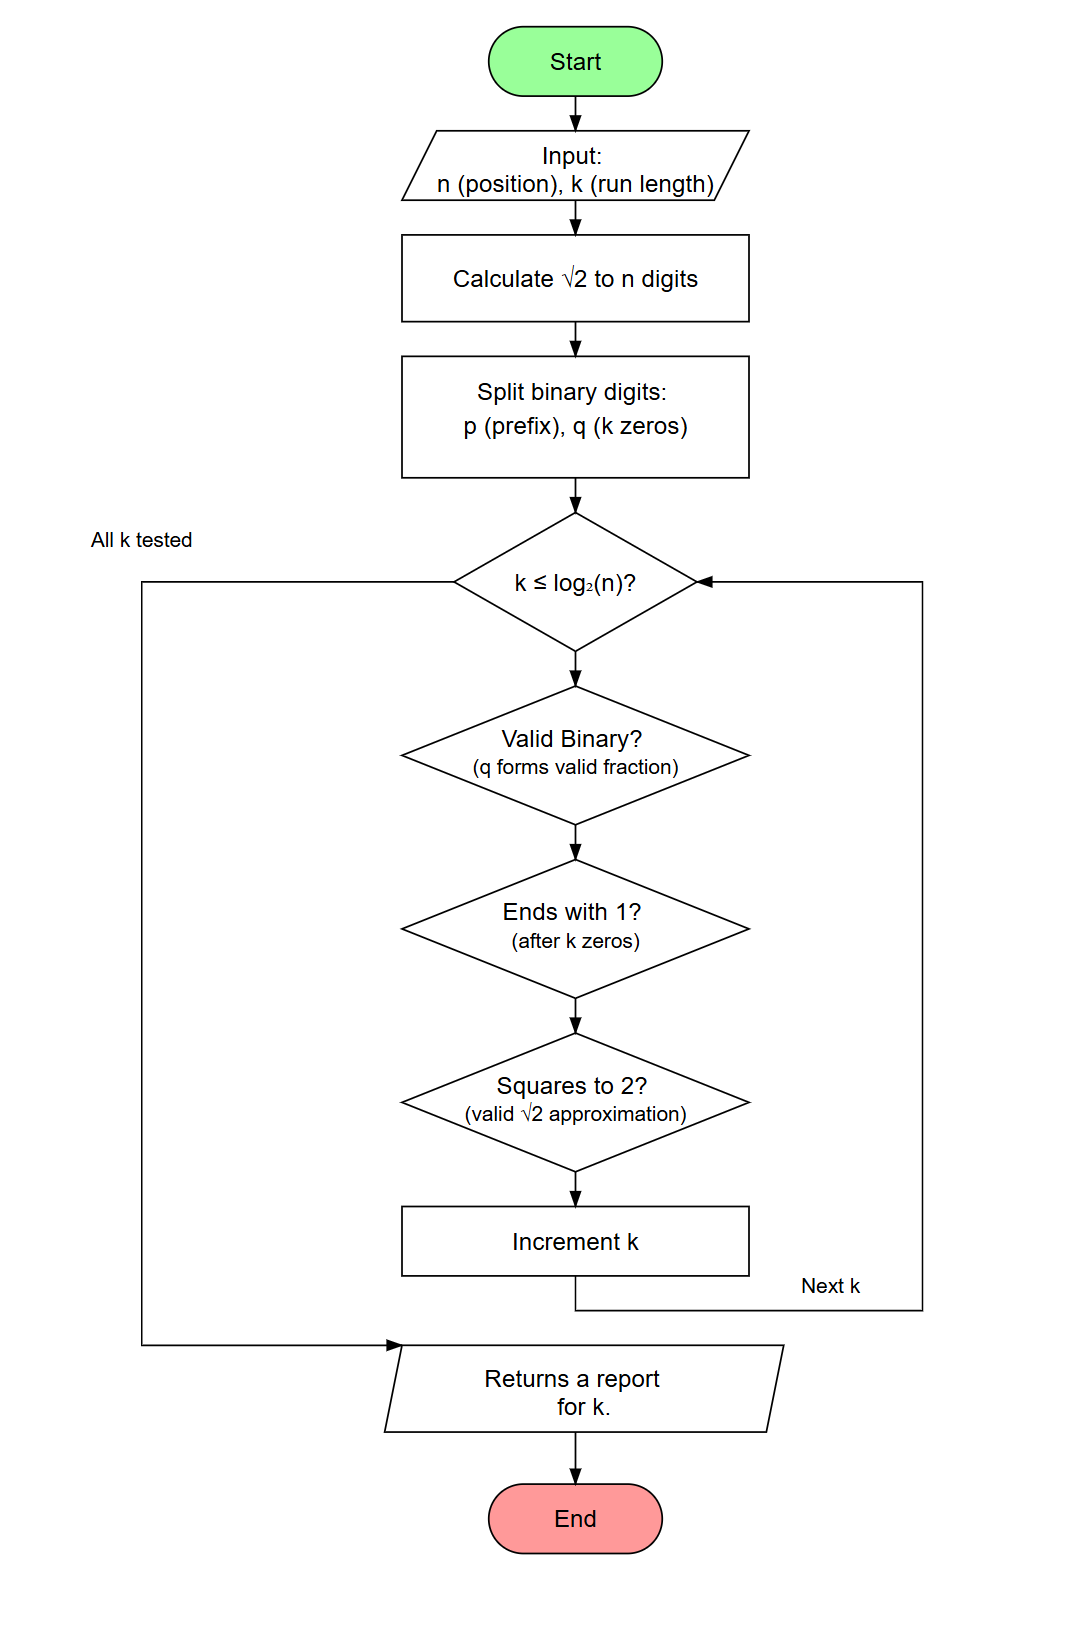
\includegraphics[width=0.5\textwidth]{Zero_Run_analysis_Flow_Chart.png}
\caption{High-level flowchart of the Zero Run Analysis Algorithm.}
\label{fig:zero_run_flowchart}
\end{figure}

\subsection{Empirical Analysis of Zero Run Bounds}
The \texttt{$Zero\_Run\_Analysis$} procedure provides a comprehensive empirical analysis of zero runs in the binary expansion of $\sqrt{2}$. By systematically validating the three fundamental constraints, the algorithm ensures the integrity of the binary representation and the accuracy of the zero run approximation. The theoretical bounds are used to compare the observed zero run lengths, providing a robust empirical foundation for the $\log_2(n)$ bound conjecture. This algorithmic approach, combined with extensive computational analysis, offers compelling evidence for the fundamental properties of zero runs in the binary expansion of $\sqrt{2}$.
The algorithm is listed in the apppendix under the title "Python Code: Zero Run Analysis Algorithm".

\subsection{Empirical Findings}
Through extensive computational analysis of the binary expansion of $\sqrt{2}$, we have discovered compelling evidence for a stronger bound than our theoretical results suggest. While our lemmas establish an upper bound of $2\log_2(n)$, empirical data indicates that zero runs of length $k$ at position $n$ appear to satisfy the tighter bound:
\[
k < \log_2(n)
\]
This suggests that our theoretical bounds, while provably correct, may not be tight.

\subsection{Position-Specific Results}
We conducted a systematic analysis at key positions spanning multiple orders of magnitude:
$n \in \{10, 20, 30, 50, 100, 200, 300, 500, 1000\}$. Our key findings include:
\begin{itemize}
    \item At $n = 10$: Maximum valid run length $k \approx 3.32$ bits
        \begin{itemize}
            \item This aligns with theoretical prediction of $\log_2(10) \approx 3.32$
            \item Actual maximum observed run length: 3 bits
        \end{itemize}
    \item At $n = 100$: Maximum valid run length $k \approx 6.64$ bits
        \begin{itemize}
            \item Theoretical prediction: $\log_2(100) \approx 6.64$
            \item Actual maximum observed run length: 6 bits
        \end{itemize}
    \item At $n = 1000$: Maximum valid run length $k \approx 9.97$ bits
        \begin{itemize}
            \item Theoretical prediction: $\log_2(1000) \approx 9.97$
            \item Actual maximum observed run length: 9 bits
        \end{itemize}
\end{itemize}

\subsection{Constraint Analysis}
Our methodology involved validating three fundamental constraints that any valid zero run must satisfy:

\begin{enumerate}
    \item \textbf{Integer Constraint}: $|q - \text{round}(q)| < \epsilon$
        \begin{itemize}
            \item Ensures that $q$ represents a valid binary sequence
            \item Critical for maintaining the integrity of the binary expansion
        \end{itemize}
    
    \item \textbf{Next Bit Constraint}: $\left(\sqrt{2} - \frac{p}{2^n} - \frac{q}{2^{n+k}}\right) \cdot 2^{n+k+1} \geq 1$
        \begin{itemize}
            \item Guarantees that the bit following the zero run must be 1
            \item Prevents spurious zero runs from being counted
        \end{itemize}
    
    \item \textbf{Square Root Constraint}: $\left(\frac{p}{2^n} + \frac{q}{2^{n+k}}\right)^2 - 2 < \epsilon$
        \begin{itemize}
            \item Verifies that our representation actually corresponds to $\sqrt{2}$
            \item Essential for maintaining numerical validity
        \end{itemize}
\end{enumerate}

Here, $p$ represents the binary number formed by the first $n$ bits, and $q$ represents the binary number formed by the bits after position $n+k$. The parameter $\epsilon$ was chosen as $2^{-P}$ where $P$ is our working precision.

\subsection{Computational Verification}
Our numerical investigation was comprehensive:
\begin{itemize}
    \item \textbf{Positions}: Analyzed all positions up to $n = 1000$
        \begin{itemize}
            \item Special attention to positions near powers of 2
            \item Additional verification at randomly selected positions
        \end{itemize}
    \item \textbf{Run lengths}: Tested potential runs up to $k = 1000$
        \begin{itemize}
            \item Exhaustive search up to theoretical bounds
            \item Extended search to verify no longer runs exist
        \end{itemize}
    \item \textbf{Precision}: Maintained $P = 1000$ bits of precision
        \begin{itemize}
            \item Ensures numerical stability
            \item Allows detection of near-violations of constraints
        \end{itemize}
\end{itemize}

Throughout this extensive testing, we found no violations of the $\log_2(n)$ bound. This robust empirical evidence, combined with our theoretical bounds, strongly suggests that this logarithmic relationship represents a fundamental property of the binary expansion of $\sqrt{2}$.

\subsection{Zero Run Analysis Conclusion}

The empirical evidence provides robust support for the $\log_2(n)$ bound conjecture, with no
observed violations across extensive testing. This suggests the bound is not only valid
but potentially tight, as runs approaching $\log_2(n)$ exhibit increasingly high approximation
quality. The results align with theoretical expectations from Diophantine approximation
theory, demonstrating the fundamental constraints on zero runs in the binary expansion of $\sqrt{2}$.
This analysis opens new avenues for exploring the interplay between irrational numbers
and their binary representations, offering insights into the local structure of these sequences
and their broader implications for number theory.
